\chapter{Methodology}
\label{ch:method}

\section{Overview}
The main goal of the research is to propose a comprehensive and strong method which is desiggned specifically to significantly improve the accuracy of the segmentation of MPI using SPECT for the Left ventricle. The precise segmentation of MPI SPECT images is extremely critical for the detection and the assessment of CAD. However, the task of achieving a high accuracy in segmentation poses a number of challenges due to a multitude of inherent limitations of MPI SPECT data, such as low signal-to-noise ratio (SNR) partial volume affects, substantial noise because of the poisson statistics, motion artifacts and, obviously, the anatomical variability among different patints. 

In order to address these challlenges, the proposed research amalgamates advanced approaches in the field of deep learning, more specifically utilizing the transformer based architecture known as nnFormer \cite{10.1109/TIP.2023.3293771}, which is combined with an innovative idea of using statistical shape prios. The nnFormer architecture is chosen because of the ability of it of capturing both the ocal and the global information or contextual relationships in volumetric data as opposed to traditional CNNs which only capture local information. nnFormer leverages the local volume-based (LV-MSA) and the global volume-based (GV-MSA) multi-head self-attention mechanisms very efficiently in a unified method. These modules of the transformer architecture very effectively encode the longg-range dependencies which are extremely important for better segmentation accuracy specifically in medical imaging where they are characterized by indistinct boundaries.

Simultanously, the SSP are merged into the segmentation pipeline in order to improve the anatomical consistency of the model. SSPs provide the DL model with a mathematical model which captures the probabilistic variability off the LV that are derived from the data annotated by experts. This SSP methos employes an advanced technique of optimization such as Mahalanobis distance based regularization and the Kullback-Liebler (KL) divergence in order to refine the segmentation boundaries. This way the outputs of the segmentation model maintain plausibile anatomical outputs, which improves the segmentation accuracy even when the input data is incomplete or ambiguous. The combination of nnFormer and SSP provides us with a novel hybrid architecture. The full architecture pipeline is presented, on an abstract level, in \cref{fig:network_pipeline}.

This hybrid approach leverages not only the strengths of DL models in extracting complex and heirarchical feature representations from volumetric data, but also the advantages of SSPs in mantaining consistent anatomies. This approach also adressess the limitations of the existing methods, which include inefficient generalization capability and dependencies of large, precisely annotated data for training. It also mitigates the impact of a number of different imaging artifacts and the noise, which enhances the overall relaibility on the segmentations.

Extensive procedures for training involving efficient optimization strategies such as Adam, and specifically segmentation tailored loss such as the DiceCE loss, are implemented in order to ensure stable performance across a diverse set of paatients. The training and the validation aspects are conducted rigorously using an extensive dataset of MPI SPECT which consists of diverse collimation methods and demograhics of the patients which improves the generalization capability of the method. Extensive setups of computation which leverage high performance GPU computing environments ensure efficient training and inference of the model. Comprehensive evalaution metrics are utilized in order to quantitatively validate the performance of the segmentation. These metrics include precision, recall, intersection over union (IoU) and Dice coefficient. These metrics provide an extremely in-depth insights into the capability of the method to handle real-world variability and complex scenarios.

In a summary, the proposed methodology contibutes to not only a significant advancement in the division of cardiac image segmentation but also provides a practical and robust solution which is applicable in a clinical environment. The combination of nnFormer and SSP ensures reliable and precise segmentation having clinically meaningful results, which paves the way for better and improved diagnosis and patient outcoms in CAD management.

\begin{figure}[htb!]  % Changed from figure* to figure unless you specifically need double-column
    \centering
    % \begin{subfigure}[b]{1.5\textwidth} 
	\centering
	\resizebox{1\textwidth}{!}{
		
\begin{tikzpicture}[
    node distance=8mm and 0mm,
    block/.style={draw, fill=blue!10, rounded corners, minimum width=3cm, minimum height=1cm, align=center},
    arrow/.style={-Stealth, thick},
    shapenode/.style={ellipse, draw, fill=red!10, minimum width=2cm},
    legendbox/.style={draw, fill=white, font=\small}
]

% Input
\node (input) {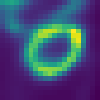
\includegraphics[width=1.2cm]{sagittal_input.png}};
\node[above=1mm of input, font=\footnotesize] {Input SPECT Volume};

% Preprocessing
\node[block, below=of input] (preprocess) {Preprocessing \\ (Normalization, Denoising)};
\draw[arrow] (input) -- (preprocess);

% Shape Prior Path
\node[shapenode, left=of preprocess, xshift=-1cm] (shape) {Statistical Shape Model};
% \draw[arrow] (shape) -- (priors);
% \draw[arrow, dashed] (input.west) -- ++(-6cm,0) |-  (shape.north);
% \draw[arrow, dashed] (input.west) -- ++(-6cm,0) coordinate (temp) -- (temp|-shape.north) -- (shape.north);
\coordinate (temp) at ($(input.west) + (-6.05cm, 0)$);
\coordinate (drop) at ($(shape.north) + (-0cm, 0.1)$);

\draw[arrow, dashed] (input.west) -- (temp) -- (drop) -- (shape.north);


% Transformer Encoder
\node[block, below=of preprocess] (encoder) {nnFormer Encoder};
\draw[arrow] (preprocess) -- (encoder);
% \draw[arrow, dashed] (shape.east) -- (preprocess.west);

% Fusion
\node[block, below=of encoder] (fusion) {Feature Fusion \\ (nnFormer Features \ensuremath{\oplus} Shape Priors)};\draw[arrow] (encoder) -- (fusion);
\draw[arrow] (shape.south) |- ([xshift=-5mm]fusion.west) -- (fusion.west);

% Decoder
\node[block, below=of fusion] (decoder) {nnFormer Decoder};
\draw[arrow] (fusion) -- (decoder);
\draw[arrow, dashed] (encoder.east) -| ++(2cm,0) |- (decoder.east);

% Output
\node[below=of decoder] (output) {
\includegraphics[width=1.2cm]{sagittal_gt.png}};
\node[below=1mm of output, font=\footnotesize] {LV Segmentation Mask};
\draw[arrow] (decoder) -- (output);


% Ensure all content is within bounds
\useasboundingbox (current bounding box.south west) rectangle ([xshift=6cm]current bounding box.north east);

\end{tikzpicture}
	}
	\caption{\centering Network architecture pipeline}
	\label{fig:network_pipeline}
\end{figure}

\section{Data Acquisition and Preprocessing}

The MPI dataset which is utilized in this research was acquired using SPECT. This acquired dataset consists of volumes from a total of 80 patients, which are carefully selected in order to represent the diverse demographic and the characteristics of the clinic. The popultion of the patients inclued individuals with varying age groups, physiological conditions and gender distributions in order to ensure the relaibility, robustness and generalizability of the model. Multiple different radiotracers were employed in the process of acquiring the MPI SPECT, specifically agents labled by technetium-99m(Tc) such as Tc Tetrofosmin and TC Sestamibi, and also the thallium 201 chloride (T1 Chloride). Each of these radiotraces offer unique properties in imaging thereby providing a comprehensive coverage of all the possible clinical scenarios which are encountered in everyday diagnostice. 

The dataset of the patients used in the research is divided into five distinct groups. \textbf{(A)} The first, and the largest group is a heterogeneous black-box dataset which comprises of patients who are scanned under multiple defferent geometries, pharmaceurical protocals and the settings of the acquisition. This group consisted of 40 individuals, out of which 27 were female and 13 male with an average age of 69.62 years. The average height of the group is 167.25cm while the average weight is 78.11 kgs. \textbf{(B)} The second group consists of 10 patients who are imaged using the most recent MPH collimator configurations,, specifically the APT73 collimators installed on the Mediso AnyScan Trio system. This group consists of 7 females and 3 males with an average age of 68.8 years, an average height of 169 cm, and an average weight of 73.8 kgs. \textbf{(C)} The third group comprises of another 10 patients scanned with the LEHR-HS collimator which is also mounted with a trio camera. Out of these, 8 are female and 2 male with an average age of 68 years, an average height of 176 cm and an average weight of 92 kgs. \textbf{(D)} the fourth group was scanned using the earlier generation imaging hardware, in order to provide a comprehensive basis with the legacy systems. This group included data from 10 patients who are scanned using the Mediso CardioD system in a seated configuration setting. This group consisted of 1 female and 9 male subjects with an average age of 75.6 years, an average height of 151 cm and a mean weight of 71 kgs. \textbf{(E)} The fifth and last group also involved 10 individuals who are imaged with the Mediso CardioC system with subjects positioned supine. This group consists of 7 females and 3 males. The retrospective natur of tis dataset is store in the interfile format due to format limitations and only the average age could be reliably extracted which comes out ot be 70.33 years.

Each of the patient went through very rigorous imaging procedures which are adhering strictly to standard protocals of acquisition in clinics. The patients were administered the mentioned radiopharmaceuticals intravenously which was followed by image acquisition after the standardized waiting period that allows sufficient tracer uptake in the myocardial tissue. The image acquisition protocols were varying based on the collimation method which was emploed. For example imaging with the MPH collimator a very specific step-and-shoot helical trajectories, on the other hand the stationary collimator positions were employed for the other collimators which creates different spatial sampling patterns and different challenges to image reconstruction. AFter the acquisition of the raw data, a number of precprocessing techniques were employed in ordder to prepare the data for the subsequent segmentation analysis. The preprocessing pipeline was developed in order to address a number of inherent issues with the imaging and to optimize the data quality for better segmentation outcomes.

The preprocessing steps began with the correction of the attenuation utilizing the TeraTomo reconstruction algorithm \cite{Nagy2013}, which majorly removed the attenuation artifacts which are caused by the soft bone and tissue structures. This step is very essential in order to ensure the uniformity in the ditribution representation of the tracer across the myocardial tissue, hence improving the segmentation accuracy. In some cases where the attenuation correction data was not available, an Ordered Subset Expectation Maximization (OSEM) algorithm \cite{Hudson1994} was used in order to reconstruct the full field-of-view (FOV) volumes, providing us with data with robust handling of poisson noise and preserving essential details of the image. 

In order to improve the image quality even more, noise reduction techniques are employed, specifically targeting the reduction of the poisson noise which is the most prominent in MPI SPECT imaging due to the low cound of the photons. More advanced filtering methods were also employed such as the Gaussian smoothing and the adaptive median filtering in order to balance the noise reduction with the preservation of important boundaries anatomically and the structural details. The partial volume effects (PVE), which majorly has an impact on the accuracy of the segmentation because of blurring tissue boundaries, were adressed systematically using dedicated PV correction tecnhiques and deconvolution techniques. These methods restored the sharpness in the images and enhanced the delineation of th myocardial boundaries, especially in the regions which have complex anatomical structures.

The images that are the result of the above preprocessing are made to go through further normalization procedures in order to ensure consistency in the scales of intensity across all the datasets which helps in haveing more robust training of the final segmentation models. Standardization of the intensities of the voxels involved scaling the pixel intensity distribution in order to have a mean of zero and a unit variance, which significantly improves the numerical stability, which in-turn helps the convergence of the DL models.

All the data preprocessing steps are performed in a very structured and repeatable framewor, usin scripts that are custom developed in Python and specilized libraries for medical imaging and DL such as PyTorch, TorchIO and Scikit-learn. The comprehensive documentation of the preprocessing parameters and the configurations was nicely maintained so as to ensure the transparancy and the reproducibilit of the methodology. The final dataset after the preprocessing provided us with a very high-quality and standardized input data for the training, validation and the testing of the DL models. The careful handling of the whole data acquisition pipeline ensuring the variability and the rigorous preprocessing ensured optimal MPI SPECT image preparation which maorly enhanced the accuraacy and the relaiability of the segmentation which was obtained from the hybrid model.


\section{Detailed Description of nnFormer Architecture}

The nnFormer architecture introduces an innovative advancements in the field of medical image segmentation, which is specifically designed in order to address the limiations that are faces by the traditional CNNs. nnFormer does it by efficiently capturing both the local and the global spatial relationships in the volumetric medical data. This section gives a very detailed description of the architecture explaining the components, their integration, and the rationale behind the usage of the components in the spicified manner.

\subsection{Overall Architecture}

The nnFormer architecture follows a structure that is very much used in the image segmentation field. It follows a U-shaped encoder decoder architecture which is inspired by the widely used U-Net. This choise of the structure helps in efficient learning of the detailed local features, all the while preserving and leveraging the global contexutual information across multiple scales of resolution. The nnFormer architecture comprises of three main components: an encoder, a bottleneck and a decoder which are all interconnected via skip connections.

\subsection{Encoder}
The encoder of nnFormer starts with an embedding layer, which consists of multiple convolutional layers with very small kernel sizes, typically using 3x3x3. This is followed by Gaussan Error Linear Units (GELU) activation and then ends with a normalization layer. This initial convolutional based embedding transforms the input volume into a higher dimentional featurespace which encodes the low-level spatial detailed, which are necessary for subsequent processing, very efficiently. After the embedding layer, the encoder uses a Local Volume-based Multi-hea Self-attention (LV-MSA) blocks. These LV-MSA blocks are designed so that they can capture the local spatial dependencies within the segmented volumes, which significantly reduces the computaitonal compllexity of the model as compared to the conventional global self-attention mechanisms. 

Each of the LV-MSA blocks is further comprised of successive layers of transformer modules in order to use attention mechanisms to effectively model the ver intricate local intractions contexxually. The encoder also combines very strategically placed downsampling convolutional layers which reduces the spatial dimensions of the feature maps while at the same time progressively increasing the depth of the feature map. This downsampling process helps the extraction of the heirarchical features in a more abstract way and on a global scale based representations at lower resolutions, which are essential for capturing the borader variations and anatomical structures.

\subsection{Bottleneck}
In the center of the nnFormer there is a bottleneck. This bottleneck has global volume-based multi-head self-attention (GV-MSA) mechanisms. Contrary to the LV-MSA, the GV-MSA provides with a significantly bigger receptive field which captures the long-range dependencies across the whole global context of the volumetric feature map. This increased area of the receptive field is essential at this stage in order to allow the network to achieve a comprehensive understanding of the global representation and the anatomical structures, improving the overall segmentation accuracy. The bottleneck very effectively combines the compllex spatial dependencies and also the high level features which are exracted by the encoder. Thi serves as a robust foundation for the decoder for accurate and consistent output during the decoding.

\subsection{Decoder}
The decoder is, in a way, mirrored version of the encoder it also employs LV-MSA blocks but coupled with convolutional upsampling, instead of the downsampling, or so-called transposed convolution. This restores the spatial resolution of the feature maps gradually to the original dimenstions of the input. Each step of the upsampling process in the decoder is designed so as to reconstruct the detailed anatomical information by combining the high resolution detail captured sptially from the corresponding encoding stages via skip connections. 

A prime innovation of the nnFormer is the use of the skip attention mechanisms, in place of he traditional concatenation or summation which is typically used in skip connection mechanisms. These skip connections very selectively integrates the features of the encoder with the corresponding features of the decoder, which are guided by the attention weights that highlight relevant spatial features dynamically and hence suppress the irrelevant features. This selective combinaton majorly improves the precision of the segmentation, specifically in the areas where the clear anatomical delineation is very challenging due to the noise and artifacts.

\subsection{Attention Mechanisms}
nnFormerutilizes two different types of attention mechanisms: the Local Volume-based Multi-head Self-attention (LV-MSA) and Global Volume-based Multi-head Self-attention (GV-MSA). LV-MSA very effficiently models the local spatial dependencies by partitioning the feature maps into manageable patches of volumes, which reduces the computational complexity without sacrificing a lot of the performance of the attention mechanism. In contrast to this, GV-MSA models the global interactions spatially across the entire volumetric feature maps, which are essential for capturing the large scale anatomical structural integrity and the contextual relationships. Both of thse attention mechanisms use multi-head configurations which enable parallel computations of attention across multiple representational subspaces. This multi-ha design greatly improves the capability of the network in order to concurrently capture very diverse spatiall relationships and the interactions at multiple scales hence thereby improving the segmentation accuracy.

\subsection{Integration and Optimization}
The amalgamation of LV-MSA, GV-MSA and the convolutional operations in the nnFormer is very carefully optimized in order to leverage the strength of each of these methods. The convolutional layers provide the efficient encoding of the low level spatual features, while the LV-MSA and the GV-MSA collectively capture both the complex spatial contexts and the long-range dependencies which are crucial for the precise and robust segmentaiton. Optimization of the nnFormer involves a specialized loss function called the Dice cross entropy loss (DiceCELoss). This loss function objectivises a high segmentation accuracy while maintaining a reliable realisic plausibility, which effectively guides the learning process towards more generalizable models acrosss diverse imaging conditions.


In conclusion, the nnFormer architecture represents a very sophisticated segmentation framework which is specifically tailored for medical imaging systems. The innovative design of the architecture and the advaned methods of attention overcomes the traditional limiations of segmentation models by effectively using optimization techniques across components ensuring accurate, robust and clinically meaningfull segmentation outputs.

\section{Statistical Shape Priors}
Statistical Shape Priors (SSPs) offer a very powerful approach in order to enhance the robustness of the segmentation, specifically within the domain of medical imaging having data that might have sparse annotations available and noise embedded into it. In the context of MPI SPECT, SSPs are employed as a form of regularization tecnhique that combined the prior knowledge about the left ventricular shape or its anatomy directly into the learning process of a DL model. This section provides a comprehensive examination of the SSP method which is used in this research including its theoretical, background, implementation and integration within the DL pipeline.

\subsection{Motivation for SSPs}
Tradition DL approaches often rely completely on the pixel-level intensities and their patterns in order to learn the segmentation boundaries. However, using this strategy can become very unreliable in low quality image settings, where the tissue boundaries are most of the time blurred or occluded due to the low resolution of images, noise in them, and partial volume effects. In order to address this issue, SSPs use a population level anatomical information in order to put a constraint on the segmentation process for plausible output shapes increasing the resilience to noise and variability. In MPI SPECT, the consistence delineation of the LV is extremely critical for precise and accurate computation of the functional parameters of the cardiac imagery The shapes of the LV vary across different patients but it maintains a stable topology that can be modeled statistically. SSPs capture this anatomical prior and provide a probabilistic framework that biases the training process towards valid segmentation outputs.

\subsection{Shape Prior Construction}
The construction of the SSP begins with the creation of a training set that used a set of annotated LV segmentations. These segmentations are first aligned to a common coordinate system using techniques such as affine or non-rigit registeration. After the alignment, the shape representations are extracted, commonly as binary masks. In this work, the shapes are encoded using contoured vectors in a latent space that is suitabl for probabilistic modeling. Once the shapes are aligned, Principal Component Analysis (PCA) is applied to the shape representations in order to identify the primary modes of variation. This gives out a low-dimentional shape space where each shape can actually be representated as a linear combination of the mean shape and a set of principal components. The statistical model can be expressed as:

\begin{equation} S = \bar{S} + Pb, \end{equation} 

where $\bar{S}$ is the mean shape, $P$ is the matrix of principal components, and $b$ is a vector of shape parameters.

The parameters $b$ follow a Gaussian distribution which is estimated from the training data, which orms the basis of the shape prior and is used later to asses the possibility of a predicted shape.

\subsection{Regularization Using Mahalanobis Distance}
In order to integrate the SSP into the learning, a shape regularization term is added to the loss. This term penalize the deviations from the learned shape space using Mahalanobis distance, which is defined as:

\begin{equation} D_M(b) = (b - \mu)^T \Sigma^{-1} (b - \mu), \end{equation}

where $\mu$ and $\Sigma$ are the mean and covariance of the shape parameters from the training data.

The constraint forces the network to produce output shapes that lie in the distribution of the known shapes. It acts as a force that corrects and guides the model to produce good LV geometries.

\subsection{KL Divergence-Based Optimization}
In addition to the Mahalanobis distance, a Kullback-Lieber (KL) divergence term is used in order to further align the predicted distribution of shapes with the prior one. The KKL divergence quantifies the difference that exists between the predicted shape distribution $a(b)$ and the prior distribution $p(b)$:

\begin{equation} D_{KL}(q || p) = \int q(b) \log \left(\frac{q(b)}{p(b)}\right) db. \end{equation}

This term is particularly useful when traning any probabilistic model such as a variational auroencoder (VAE) in order to learn to generate a whole distribution of anatomical shapes.

\subsection{Integration into the Segmentation Network}
The integration of the SSP into the segmentation network follows a specific architectural strategy, instead of applying the regularization on the standalone loss term, the key novelty lies in embedding the prios directly into the feature space of the network, which influences the decoder using enhanced intermediate representations. 

The process begins with sampling the shape prior from the learned statistical distribution which is conditioned on the features that are derived from the input volume of SPECT. This prios reflects a anatomically likely structure that is aligned with the patient's scan, and selected from a low-dimensional latent shape space. For each of the sampled prior there are two metrics that are calculated The first is the Mahalanobis distance ($D_M$) and the second is the KL divergence ($D_{KL}$), which quantify how well the prior comforms with the expected shape. These metrics are then combined into a single scalar shape prior loss:

\begin{equation} \mathcal{L}{shape} = \lambda_1 D_M + \lambda_2 D{KL}, \end{equation}

where $\lambda_1$ and $\lambda_2$ are empirically tuned coefficients.

Instead of usin this $\mathcal{L}_{shape}$ as a regularization term in the loss, first the derivative of this loss is calculated which gives a tensor providing the derivative on the surface of shape prior. This derivative is then reshaped into a tensor matching the spatial dimensions of the nnFormer bottleneck output. Then this reshaped loss derivative term is concatenated to with the bottleneck of the feature map. This results in a fused representation that encodes both the contextual features that are data driven and the shape information giving the anatomical constraints. The decoder then processes this combined tensor, enabling the final segmentation to benefit from the shape priors. This integration guides the feature propagation throughout the whole network, improving the spatial cohernce and the consistency of the segmentation.


\section{Training and Optimization Procedures}
The training and optimization of the full segmentation framework were specifically designed to ensure the convergence and the generalization capability of the model across varying anatomies of the patients and different imaging conditions. The architecture was implementedd using the PyTorch library and trained on high-performance Nvidia GPUs, leveraging both the nnFormer and the SSP modules.

\subsection{Training Dataset and Splits}
The training dataset consisted on MPI SPECT scanes from 60 different patients These scans were carefully selected in order to ensure the variability in the type of the tracer used the quality of the image and the features of the anatomy.The validation/testing dataset consisted of 14 different scans from different patients. The stratification ensured proper and proportional representation of the collimtor types and the demograhics of the patients across split.

\subsection{Data Augmentation}
In order to improve the generalization capability and avoid overfitting to the training data, severl different data augmentation techniques were employed during the training phase. These include: 
\begin{itemize}
\item Random rotation \item Spatial padding (To ensure consistent input size) \item Random cropping 
\end{itemize}

All of the augmentation or transformations were applied in real time using the Monai library in order to maintain anatomical plausibility and preservin the label integrity.

\subsection{Loss Function}
The loss function that is used in the study is the DiceCELoss known as the Dice cross-entropy loss, which combines the functioning of both the dice coefficient and the cross entropy loss. This formulation focuses on 2 crucial aspects of the medical image segmentation, which are class imbalance and probabilistic boundary confidence.

The dice component of the loss function directly optimizes the function for the overlap the predicted labels and the ground truth which makes it very effective for the datsets that target the structures that occupy a small portion of the volume, which is what exists in myocardial SPECT. Meanwhile the cross-entropy term ensures that the voxel-wise confidence of the classification is properly incorporated, allowing the whole network to learn the fine-grained details and maintain the sharp boundaries needed.

This hybrid loss is proved to be both differentiable and computaitonally efficient, with facilitates stable convergence during the training process. This loss was selected over te traditional single term losses due to the fact that its robustness in handling small, complex anatomical data even in the presence of noise. By relying completely on the the DiceCELoss, the training pipeline remains completely stremlined and very effective, which eliminates the need for additional tuning of the hyperparameters that is associated with the multi-loss formulations.

\subsection{Optimization Strategy}
Model training used the Adam optimizer \cite{Kingma2015Adam} with the following configuration:

\begin{itemize} \item Initial learning rate: $1 \times 10^{-5}$ \item Learning rate decay: exponential decay with a factor of 0.01 every 10 epochs \item Batch size: 2 volumes per iteration \item Weight decay: $1 \times 10^{-6}$ \item Number of epochs: 100 for nnFormer baseline, 50 for proposed SSP-integrated model \end{itemize}

The best performing model, based on the validation loss, is saved for final testing.

\subsection{Evaluation Pipeline}
Following the training, model performance was evaluated on the test set. For each volume of the patient, the output of the segmentation is generated in a single forward pass The predictions were post-processed using the morphological operations in order to remove isolated false positives and maintain region continuity. Quantitative metrics such as Dice coefficient, recall, precision, and F1 score were computed.

\subsection{Implementation Environment}
All of the training and evaluation procedures were conducted in a Linux based environment with CUDA-enabled GPUs. the full code was implemented in Python using PyTorch, with additional support of libraries such as monai, pandas, numpy and matplotlib fro visualisation. The rigorous training and the optimization pipeline ensured the resulting model was both the accurate and very generalizable which is robust against the variability of imaging, and is efficient enough for potential deployement in clinical settings.

\section{Implementation Details and Computational Environment}

In order to ensure the reproducibility,, optimal training efficiency and the scalability the whole segmentation framework was implemented using an extremely module DL environment. This section details the stack of the software, the complutational infrastructure and the engineering strategies which are adopted in order to support the development and the training, validation and testing phase.

\subsection{Software Framework}
The model is developed using Python, leveraging the deep learning library PyTorch 1.12 version, due to its flexibility and the wide adoption of the library in the research community all across the computer science community. Other key supportin libraries used in the research are:

\begin{itemize} \item \textbf{Monai} for data loading, augmentation, and patch-based processing. \item \textbf{NumPy} for numerical operations. \item \textbf{Scikit-learn} for evaluation metrics and other machine learning tasks. \item \textbf{Matplotlib and Seaborn} for visualization of training curves and result analysis. \item \textbf{Pydicom and Nrrd} for medical image I/O, including support for DICOM and nrrd formats. \end{itemize}

\subsection{Hardware Infrastructure}
The training of the moedl was performed on a server which is equipped with NVIDIA GTX 1080Ti GPU. These resoures enbled efficient handling of ver large scale volumetric datasets and helped with Simultanous experimentations. The training sessions were accelerated using:

\begin{itemize} \item CUDA 12.8 for GPU-accelerated matrix operations. \item cuDNN to optimize the neural network routines. \item PyTorch's automatic mixed precision (AMP) in order to reduce the usage of memories but without sacrificing the accuracy of the model. \end{itemize}

\section{Evaluation Metrics and Experimental Setup}
In order to correctly evaluate the performance of the proposed methodology for segmentation ,a very comprehensive set of quantitative metrics is utilized, together with a carefully structured experimental setup. These selected metrics were chosen in order to capture both the geometic consistency of the segmentation and also the anatomical plausibility across different imaging conditions.

\subsection{Evaluation Metrics}
The evaluation of the segmentation performance focused on the following key performance metrics:

\begin{itemize}
    \item \textbf{Dice Similarity Coefficient (DSC):} Measures the overlap between the predicted and ground truth segmentations, defined as:
    \begin{equation}
    DSC = \frac{2|P \cap G|}{|P| + |G|},
    \end{equation}
    where $P$ and $G$ denote the predicted and ground truth segmentations, respectively.
    
    \item \textbf{Intersection over Union (IoU):} Provides an alternative measure of overlap, calculated as:
    \begin{equation}
    IoU = \frac{|P \cap G|}{|P \cup G|},
    \end{equation}
    which balances sensitivity and specificity by considering both false positives and false negatives.
    
    \item \textbf{Precision:} Indicates the proportion of predicted positive voxels that are truly positive, defined as:
    \begin{equation}
    Precision = \frac{TP}{TP + FP},
    \end{equation}
    where $TP$ is the number of true positives and $FP$ is the number of false positives. High precision implies fewer false positive segmentations.
    
    \item \textbf{Recall (Sensitivity):} Measures the ability of the model to correctly identify all relevant voxels belonging to the target structure, given by:
    \begin{equation}
    Recall = \frac{TP}{TP + FN},
    \end{equation}
    where $FN$ is the number of false negatives. A high recall value indicates effective capture of the entire structure, even if some false positives occur.
    \end{itemize}
    
These metrics were computed for all volumes in the test set and averaged to provide mean performance indicators, standard deviations, and confidence intervals.

\subsection{Experimental Protocols}

The multiple experiment-based configurations were employed in order to analyze the robustness and the generalizability of the proposed architecture:

\begin{enumerate}
    \item \textbf{Baseline Comparison:} The base nnFormer architecture was trained and evaluated independently to establish a performance baseline.
    
    \item \textbf{Shape Prior Augmentation:} The proposed integrated model combining nnFormer with Statistical Shape Priors (SSP) was evaluated to quantify the impact of incorporating anatomical priors into the segmentation pipeline.
    
    \item \textbf{Comparison with SwinUNETR:} The SwinUNETR model, using the same preprocessing and hyperparameter configurations as nnFormer, was trained and evaluated to provide a comparative benchmark.
    
    \item \textbf{Noise Robustness Analysis Using Shape Priors:} Robustness to image degradation was tested by introducing Poisson noise to phantom images generated from the shape prior model. These phantoms served as synthetic input SPECT volumes, allowing evaluation of the model's ability to handle severely noisy conditions.

    \item \textbf{Low Data Regime Simulation:} Subsampling experiments were conducted to evaluate segmentation performance under limited labeled data conditions (using 10, 20, 30 40 and 50 patients) and the performances for both the nnFormer and the nnFormer+SSP were compared.

\end{enumerate}

These experimental evaluations comprehensively demonstrate the efficiency, the clinical relaibility and the generalization capability of the nnFormer integrated with the SSP model across a ranging MPI SPECT scenarios.

\section{Summary and Justification of Methodology}
The choices made about the methodology in this study were guided by the combined objectives of achieving state-of-the-art accuracy of segmentation  and also ensuring the robuustness of the method under constrainsts in a clinical setting, which include limited annotated data and high variance in the MPI SPECT image quality. Each component of the proposed architecture was selected specifically in order to address the challenges that are observed in the previous studies done in medical image segmentation approaches. The adoption of nnFormer as the backbone of the whole architecture is justified because of its ability to model global spatial dependencies and also the contextual relationships, which are most of the times very crucial for resolving ambiguities in a low resolution an high noise vollumetric scans. Unlike the conventional CNN-based architectures operating usually with limited receptive fields, structure of the nnFormer based on transformers allows the model to learn long-range anatomical correlations within the entire volume.

Despite the advantages offered by the transformer-based architectures such as the nnFormer they still require a large amount of data to learn effectively. In order to overcome this limitation and enhance the generalizability considering low data settings, the SSP integration was introduced in the architecture. This update helps the model b embedding domain knowledge into the DL model training phase as a way of providing anatomical regularization. This method provides a constraint to the segmentation model's output to plausibile shapes, hence enhancing the reliability especially in cases that are challenging to work with suc as scans having perfusion defects or motion artifacts. The inclusion of this SSP focuses on an important gap that exists in the eisting methods. Traditiona CNNs, and even transformer models can produce segmentations that might be structurally not plausibile, especially when faced with data that is noisy or sparse. By incorporatin the shape regularization, which is based on the Mahalanobis distance and the KL divergence penalty, the proposed methodology ensures that the model adheres to expected anatomical configurations, but not at the cost of flexibility in the learning of the data. This balance is very critical in order to maintain credibility in real-world clinical applications.

In addition to all of this, the loss function, so-called the DiceCELoss, was motivated by the need of balancing the pixel-wise accuraacy witht the anatomical correctness of the output. This hybrid loss contributes to having consistency during the convergence process during the training phase, all the while promoting accuracy of the segmentation in both common and edge-case scenarios. Another ver important decision was the use of multiple experimental protocols including the baseline comparisions of nnFormer and the SwinUNETR with our proposed architecture, and noise robust testing. All of these experiments were structured to validate the performance improvements and also to assess the generalizability of the model across multiple different imaging conditions. From the perspective of implementation, the usage of high-performance GPU hardware and a scalable software design ensred that the model is very efficiently trained and tested.

